%% $Id$
%% badros-javaml-www9.tex
%%
%% for:
%% Ninth International World Wide Web Conference (WWW9)
%% http://www9.org
%% Amsterdam, The Netherlands
%%
%% Final submission deadline 1-March-2000
%%

\documentclass{article}
\usepackage{graphicx}
\usepackage{fullpage}
\usepackage{times}
\usepackage{url}
\usepackage{moreverb}
\usepackage[english]{babel}
\usepackage{floatflt}
\usepackage{multicol}

\setlength\topmargin{-0.25in} \setlength\oddsidemargin{-0.25in}
\setlength\textheight{9.0in} \setlength\textwidth{7.0in}
\setlength\columnsep{0.375in}  \newlength\titlebox \setlength\titlebox{2.25in}
\setlength\headheight{0pt}   \setlength\headsep{0pt}
\setlength{\parskip}{2pt}
%\flushbottom \twocolumn \sloppy

\begin{document}
\bibliographystyle{plain}
\newcommand{\smtexttt}[1]{{\small\texttt{#1}}}
\newenvironment{smverbatim}{\small \begin{verbatim}}{\end{verbatim}}
\newenvironment{shellcommand}{\begin{verbatim}}{\end{verbatim}}
\newenvironment{shelloutput}{\begin{verbatim}}{\end{verbatim}}

\title{JavaML: A Markup Language for Java Source Code}
\author{Greg J. Badros\thanks{Corresponding author: \smtexttt{gjb@cs.washington.edu}}
\\ \small
Dept.\ of Computer Science and Engineering, ~
University of Washington, Box 352350, ~
Seattle, WA ~ 98195-2350, USA}
\date{}

%\pagestyle{empty}

\maketitle
\thispagestyle{empty}

%% GJB:FIXME:VISUAL
\vspace*{-1cm}

\section*{Abstract}
The classical plain-text representation of source code is convenient for
programmers but requires parsing to uncover the deep structure of the
program.  While sophisticated software tools parse source code to gain
access to the program's structure, many lightweight programming aids
such as \smtexttt{grep} rely instead on only the lexical structure of
source code.  I describe a new XML application that provides an
alternative representation of Java source code. This XML-based
representation, called JavaML, is more natural for tools and permits
easy specification of numerous software-engineering analyses by
leveraging the abundance of XML tools and techniques.  A robust
converter built with the IBM Jikes Java compiler framework translates
from the classical Java source code representation to JavaML.

%% GJB:FIXME:VISUAL
\vspace*{.2cm} 
\noindent \textit{Keywords:}
Java, source-code, SGML, XML, abstract syntax tree, AST, parsing,
analysis, software-engineering, Jikes

\begin{multicols}{2}

\section{Introduction}
\label{sec-intro}

Since the first computer programming languages, programmers have used a
text representation as the medium for encoding software structure and
computation.  Over the years, techniques have been developed that
largely mechanize the front-end of compilers which perform the lexical
analysis and parsing necessary to uncover the structure of programming
language constructs represented as plain text.  Tools such as Lex/Flex
and Yacc/Bison~\cite{Levine92} automate these tedious tasks by using
well-founded concepts of regular expressions and grammars. Regular
expressions describe how individual characters combine to form tokens,
and the grammar enumerates how higher-level constructs are composed
recursively of other constructs and primitive tokens.  Together, these
procedures convert from a sequence of characters into a data structure
called an \emph{abstract syntax tree} (AST) which more directly reflects
the structure of the source program.

The textual representation of source code has several nice properties.
It can be concise and is similar to natural languages, often making it
easy to read.  Text is a universal data format thus making source code
easy to exchange and manipulate using a wide variety of tools including
text editors, version control systems, and command pipeline utilities
such as \smtexttt{grep}, \smtexttt{awk}, and \smtexttt{wc}.

Nevertheless, the classical source representation has numerous problems.
The syntax of popular contemporary languages such as C++ and Perl push
the limits of parsing capabilities.  Constructing a front-end for such
languages is difficult despite the support from tools.  Perhaps more
disconcerting is that evolving the syntax of the language often requires
manipulating a fragile grammar.  This limitation complicates handling an
evolving language.

Another problem with the classical representation is that parsing is not
very robust.  A small change in the source code can have a dramatic
effect on the resulting AST and, thus, the semantics of the computation.
For example, a single extraneous semicolon can change a looping block
into an ordinary one and result in an infinite loop:

{\small
\begin{verbatim}
  int i = 10;
  while (i > 0); {
    /* ... */ --i;
  }
\end{verbatim}
}

Other, more concise, languages may suffer from far more dangerous
semantic changes stemming from small syntactic errors (the Perl language
is the infamous example).

\subsection{Text representation and software tools}

Probably the most significant limitation of the classical source
representation is that the structure of the program is made manifest
only after parsing.  This shortcoming forces language-specific parsing
functionality to be duplicated in every tool that needs to reason about
the program beyond its lexical nature.  Compilers, by necessity, must
work with the AST, but numerous other software-engineering tools would
perform better with access to the structured representation of the
source code.  Unfortunately, many software-engineering tools do not
embed a parser and thus are limited to lexical tasks.

There are several reasons why tool developers often avoid embedding a
parser in tools.  As mentioned previously, building a complete front-end
is challenging for syntactically-complex languages.  Although re-using
existing infrastructure (e.g., the grammar definition) simplifies
implementation, working with the resulting AST is not always intuitive.
An AST typically reflects quirky artifacts of the grammar rather than
representing the programming-level constructs directly.  Additionally,
embedding the front-end of a compiler may be deemed overkill when
targeting a simple analysis that can do "well enough" with lexical
information.

Other complications arise if a transformation of the source code is
desired: a change in the AST must ultimately be reflected in the
classical source representation because that is the primary long-term
storage format.  Recreating a text representation from an AST is most
straightforwardly done using an unparsing approach that can create
undesired lexical side effects (e.g., changes in indentation or
whitespace) that confuse the other lexical tools that a developer relies
upon (e.g., a version control system that is unable to disambiguate
between a meaningful change and a gratuitous one effected
unintentionally).  Finally, using a parser in a tool necessarily targets
that tool to a specific language, thus reducing its applicability and
generality.  Worse, because there is no standard structured external
representation of a source program, supporting inter-operability of
independent tools even targeting the same programming language is very
difficult.

The end result of these complications is that developers often use
simple, lexically-oriented tools such as \smtexttt{grep} or
search-and-replace within an editor.  This approach sacrifices accuracy:
imagine wanting to rename a local variable from \smtexttt{result} to
\smtexttt{answer}.  With simple search-and-replace, all occurrences of
the word will be changed, even if they refer to characters inside
comments, literal strings, or an unrelated instance field.

An alternate route taken by some developers is that they rely instead on
a fixed set of tools provided within an integrated development
environment (IDE) that has access to the structure of their source
program via an integrated language-specific parser.  This approach
sacrifices flexibility.  IDEs generally provide only a limited set of
capabilities and extending those is hard.  Additionally, analyses and
transformation on source code are often hard to automate or perform in
batch using existing interactive environments.  Some more advanced IDEs,
such as IBM VisualAge for C++~\cite{Soroker97}, expose an application
programming interface to the representation of the program.  Although an
improvement, this technique still suffers from an inability to separate
simple tools from a complex environment and additionally creates a
dependency on proprietary technology that may be undesirable.

\subsection{A solution}

One of the fundamental problems underlying the above difficulties is the
lack of a canonical structured representation of the source code.  We
need a universal format for directly representing the structure that
software tools can easily analyze and manipulate.  The key observation
is that XML, the eXtensible Markup Language~\cite{XML}, provides exactly
this capability and is an incredibly empowering complementary
representation for source code.

In this paper, I introduce the Java Markup Language, JavaML---an XML
application for describing Java source programs.  The JavaML document
type definition (DTD) specifies the various elements of a valid JavaML
document and how they may be combined.  There is a natural
correspondence between the elements and their attributes and the
programming language constructs they model.  The structure of the source
program is reflected in the nesting of elements in the JavaML document.
With this representation, we can then leverage the wealth of tools for
manipulating and querying XML and SGML documents to provide a rich
infrastructure for software engineering transformations and analyses on
Java source code.

JavaML is well-suited to be used as a canonical representation of Java
source code for tools.  It shares most of the strengths of the classical
representation and overcomes many weaknesses.  The next section
describes relevant features of Java and XML and section~\ref{sec-javaml}
details the markup language and the implementation of a converter from
the classical representation to JavaML.  Section~\ref{sec-leveraging}
gives numerous examples of how existing XML and SGML tools can be
exploited to perform source code analyses and transformations on the
richer representation provided by JavaML.  Sections~\ref{sec-related}
and \ref{sec-future} describe related work and suggest avenues for
exciting future work, and section~\ref{sec-conclusion} concludes.  The
full document type definition (DTD) for JavaML appears in
appendix~\ref{app-javaml-dtd} and an example of converted source code is
given in appendix~\ref{app-ext-eg}.

\section{Background}
\label{sec-background}

The Java Markup Language is influenced by and benefits from numerous
features of the two technologies it builds a bridge between: Java and
XML.

\subsection{Java}
\label{ssec-java}

Although the XML-based representation of programming language constructs
is language independent and could be applied to many conventional
languages, Java is an excellent candidate for experimenting with these
ideas and techniques.

Java is a popular object-oriented programming language developed by Sun
Microsystems in the mid-1990s~\cite{Arnold98,Flanagan97}.  It features a
platform-independent execution model based on the Java Virtual Machine
(JVM) and owes its quick acceptance to its use as a programming language
for World Wide Web applications.  Java combines a simple object model
reminiscent of Smalltalk~\cite{Goldberg89} with Algol block structure, a
C++-like~\cite{Stroustrup97} syntax, a static type system, and a package system
inspired by Modula-2~\cite{Modula2}.

As in most other object-oriented (OO) languages, the primary unit of
decomposition in Java is a \emph{class} which specifies the behaviour of
a set of objects.  Each class can define several \emph{methods}, or
behaviours, similar to functions or procedures. A class can also define
\emph{fields}, or state variables, that are associated with "instances"
of the class called \emph{objects}. Classes can inherit behaviour and
state from \emph{superclasses}, thus forming a hierarchy of
inter-related classes that permits factoring related code into classes
at the top of the hierarchy, and encourages re-use.  Behaviours are
invoked by sending a \emph{message} to a target receiver object that is
a request to execute a method defined for that class.  Choosing what
method to execute in response to a message is called \emph{dynamic
  dispatch} and is based on the run-time class of the object receiving
the message.  For example, an instance of the \smtexttt{ColoredBall}
class may respond to the \smtexttt{draw} message differently than an
instance of a \smtexttt{Ball} class.  This ability to behave differently
upon receipt of the same message is largely responsible for the
extensibility benefits touted by the OO community.
    
%% Java also is free from "parsing state" like "public:" and "private:" in c++

Java is being widely used both in industry and in education, and it
remains popular as a programming language on the web.  Unlike C++, a
Java class definition exists in a single, self-contained file.  There
are no separate header files and implementation files, and Java is
largely free from order-dependencies of definitions.  A method body
(when present) is always defined immediately following the declaration
of the method signature.  Additionally, Java lacks an integrated
preprocessor.  These features combine to make Java source programs
syntactically very clean and make Java an ideal language for
representing using XML.\footnote{The applicability of this approach to
  other languages is discussed further in section~\ref{sec-future}.}

\subsection{XML: Extensible Markup Language}

XML is a standardized eXtensible Markup Language~\cite{XML} that is a
subset of SGML, the standard Generalized Markup Language~\cite{SGML}.
The World Wide Web Consortium (W3C) designed XML to be lightweight and
simple, while retaining compatibility with SGML.  Although HTML
(HyperText Markup Language) is currently the standard web document
language, the W3C is positioning XML to be its replacement.  While HTML
permits authors to use only a pre-determined fixed set of tags in
marking up their document, XML allows easy specification of user-defined
markup tags adapted to the document and data at
hand~\cite{Goosens99,Goldfarb98}.

An XML document consists simply of text marked up with tags enclosed in
angle braces.  A simple example is:

\begin{verbatim}
<?xml version="1.0"?>
<!DOCTYPE email SYSTEM "email.dtd">
<email>
  <head>
    <to>Mom</to>
    <to>Dad</to>
    <from>Greg</from>
    <subject>My trip</subject>
  </head>
  <body encoding="ascii">
   The weather is terrific!
  </body>
</email>
\end{verbatim}

The \smtexttt{<email>} is an open tag for the \smtexttt{email} element.
The \smtexttt{</email>} at the end of the example is the corresponding
close tag.  Text and other nested tags can appear between the open and
close constructs. Empty elements are allowed and can be abbreviated with
a specialized form that combines the open and close tags:
\smtexttt{<\emph{tag-name}/>}.  In the above document, the
\smtexttt{email} element contains two immediate children elements: a
\smtexttt{head} and a \smtexttt{body}.  Additionally, an XML open tag
can associate attribute/value pairs with an element.  For example, the
\smtexttt{body} element above has the value \smtexttt{ascii} for its
\smtexttt{encoding} attribute.  For an XML document to be
\emph{well-formed}, the document must simply conform to the numerous
syntactic rules required of XML documents (e.g., tags must be balanced
and properly nested, attribute values must be of the proper form and
enclosed in quotes, etc.).

A more stringent characterization of an XML document is \emph{validity}.
An XML document is valid if and only if it both is well-formed and
adheres to its specified \emph{document type definition}, or \emph{DTD}.
A document type definition is a formal description of the grammar of the
specific language to be used by a class of XML documents.  A DTD defines
all the permitted element names and describes the attributes that each
kind of element may possess. It also restricts the structure of the
nesting within a valid XML document.  The preceding XML example is valid
with respect to the following DTD:

\begin{verbatim}
<!-- email DTD -->
<!ENTITY % encoding-attribute "encoding (ascii|mime) #REQUIRED">
<!ELEMENT email (head,body)>
<!ELEMENT head (to+,from,subject?)>
<!ELEMENT to (#PCDATA)>
<!ELEMENT from (#PCDATA)>
<!ELEMENT subject (#PCDATA)>
<!ELEMENT body (#PCDATA)>
<!ATTLIST body
    encrypted (yes|no) #IMPLIED
    %encoding-attribute;>
\end{verbatim}

According to this DTD, there are six element types. The \smtexttt{email}
element must contain exactly one \smtexttt{head} followed by exactly one
\smtexttt{body} element.  The \smtexttt{head}, in turn, must contain one
or more \smtexttt{to} elements and then a \smtexttt{from} element,
followed by an optional \smtexttt{subject} element.  The order of the
elements must be as specified---order \emph{does} matter. Each of those
elements may contain text (also know as \emph{parsed character data} or
\smtexttt{PCDATA}).  The single \smtexttt{ATTLIST} declaration in the
DTD specifies that the \smtexttt{body} element \emph{may} specify a
value for the \smtexttt{encrypted} attribute, and \emph{must} specify
either \smtexttt{ascii} or \smtexttt{mime} for the \smtexttt{encoding}
attribute. The \smtexttt{ENTITY} declaration of the
\smtexttt{encoding-attribute} (at the top of the DTD) is a simple way to
factor out redundant text---the text given between the quotes is
substituted as is into the following \smtexttt{ATTLIST} declaration
(and, importantly, can be used in multiple \smtexttt{ATTLIST}s).

An XML document that is declared to adhere to this DTD is not valid if
any of the above criteria are not met.  For example, if the
\smtexttt{to} element is missing from an \smtexttt{email} document, that
document is not valid, though it may still be well-formed.

When modeling data in XML, a primary design decision is choosing whether
to nest elements or to use attributes.  In the above example, we could
have folded all of the information contained in the \smtexttt{head} into
attributes of the \smtexttt{email} element if we chose.  There are
several important differences between using attributes and nesting
elements:

\begin{itemize}

\item attributes/value pairs are unordered, while nested children have a
specific order;

\item values for attributes may contain only character data, and may not
      include other markup, while nested children can arbitrarily nest
      further; and
      
\item only one value for an attribute can be given, while multiple
      elements of the same class can be included by a parent element
      (e.g., we could have multiple \smtexttt{to} elements contained by
      the \smtexttt{head} with only a simple change to the DTD).

\end{itemize}

Although the above distinctions sometimes mandate using one technique or
the other, the decision is often initially a matter of taste.  However,
later experiences using the resulting documents may suggest revisiting
the decision in order to facilitate or simplify some desired
manipulation of the document.

Another useful data modeling feature of XML is the ability to attach
unique identifiers to elements via an \smtexttt{ID} attribute.  These
elements can then be referred to by \smtexttt{IDREF} attributes of other
elements.  A well-formed XML document must have every \smtexttt{IDREF}
value match an \smtexttt{ID} given in the document.

XML, in part due to its SGML heritage, is very well supported by tools
such as Emacs editing modes, structure-based editors, DTD parsers and
editors, validation utilities, querying systems, transformation and
style languages, and many more tools.  Numerous other W3C
recommendations inter-relate to XML including Cascading Style
Sheets~\cite{CSS2}, XSL (Extensible Stylesheet Language)~\cite{XSL}, and
XSLT (XSL for Transformations)~\cite{XSLT}, XPath~\cite{XPath}, and DOM
(Document Object Model)~\cite{DOM}.

\section{Java Markup Language (JavaML)}
\label{sec-javaml}

The Java Markup Language provides a complete self-describing
representation of Java source code.  Unlike the conventional
character-based representation of programs, JavaML reflects the
structure of the software artifact directly in the nesting of elements
in the XML-based syntax.  Because XML is a text-based representation,
many of the advantages of the classical source representation remain.
Because JavaML is an XML application, JavaML is easy to parse, and all
existing tools for working with XML can be applied to Java source code
in its JavaML representation.  JavaML tools can leverage the existing
infrastructure and exploit the canonical representation to improve
inter-operability among tools.

\subsection{Possible approaches}

Although the basic approach of using an XML application to model source
code is fairly straightforward, there is a large design space for
possible markup languages.  The most obvious possibility is to simply
use XML as a textual dump format of a typical abstract syntax tree
derived from parsing source code.  Consider the simple Java program:

\begin{verbatim}
import java.applet.*;
import java.awt.*;

public class FirstApplet 
                   extends Applet {
  public void paint(Graphics g) {
    g.drawString("Hello World", 25, 50);
  }
}
\end{verbatim}

Performing the obvious (but very unsatisfying) translation from the AST
of the above might result in the below XML \emph{for just the first line
  of code}:

\begin{verbatim}
<compilation-unit>
 <ImportDeclarationsopt>
  <ImportDeclarations>
   <ImportDeclaration>
    <TypeImportOnDemandDeclaration>
      import
      <Name>
       <QualifiedName>
        <Name>
         <SimpleName>java</SimpleName>
        </Name>
        .
        <Name>
         <SimpleName>applet</SimpleName>
        </Name>
       <QualifiedName>
      </Name>
       . * ;
    </TypeImportOnDemandDeclaration>
   </ImportDeclaration>
  </ImportDeclarations>
 </ImportDeclarationsopt>
...
<compilation-unit>
\end{verbatim}

Certainly this translation is far from ideal: it is unacceptably
verbose, exposes numerous uninteresting details of the underlying
grammar that was used to do the initial parse from the classical source
representation and would be difficult to work with because of the
excessive number of nodes.

An alternate possibility is to literally mark-up the Java source program
without changing the text of the program (i.e., to only add tags).  This
approach might convert the \smtexttt{FirstApplet.java} implementation
to:

\begin{verbatim}
<java-source-program>
<import-declaration>import java.applet.*;
   </import-declaration>
<import-declaration>import java.awt.*;
   </import-declaration>

<class-declaration>
<modifiers>public</modifiers> class 
   <class-name>FirstApplet</class-name> 
     extends 
      <superclass>Applet</superclass> {
 <method-definition>
  <modifiers>public</modifiers>
        <return-type>void</return-type> 
    <method-name>paint</method-name>
      (<formal-arguments>
          <type>Graphics</type> 
          <name>g</name>
        </formal-arguments>) 
    <statements>{
    g.drawString("Hello World", 25, 50);
  } </statements>
 </method-definition>
}
</class-declaration>
</java-source-program>
\end{verbatim}

This format is a huge step towards a more useful markup language.  We
have definitely added value to the source code and it is trivial to
convert back to the classical representation: we simply remove all tags
and leave the content of the elements behind (this removal of markup is
exactly what the \smtexttt{stripsgml}~\cite{perlSGML} utility does).
Although this representation seems useful for many tasks, it still has
some problems.  First, many of the details of the code are included in
the textual content of elements.  If we want to determine what packages
are being imported, our XML query would need to lexically analyze the
content of the import-declaration elements.  Such analysis is
inconvenient and does not take advantage of the capabilities that XML
provides.  Perhaps more significantly, the above XML representation
retains artifacts from the classical source code that another
representation might permit us to abstract away from and free ourselves
of those syntactic burdens altogether.

\subsection{The chosen representation}

The prototype JavaML representation I have chosen aims to model the
programming language constructs of Java (and, indeed, similar
object-oriented programming languages) independently of the specific
syntax of the language.  One can easily imagine a SmalltalkML that would
be very similar, and even an OOML that could be converted into both
classical Java source code or Smalltalk file-out format.  With this goal
in mind, JavaML was designed from first principles of the constructs and
then iteratively refined to improve the usefulness and readability of
the resulting markup language.

JavaML is defined by the document type definition (DTD) in
appendix~\ref{app-javaml-dtd}, but is best illustrated by example.  For the
\smtexttt{FirstApplet.java} source code listed above, we represent the
program in JavaML as show in figure~\ref{fig-firstapplet-javaml}.

\begin{figure*}[htb]
\begin{listing}{1}
<?xml version="1.0" encoding="UTF-8"?>
<!DOCTYPE java-source-program SYSTEM "java-ml.dtd">

<java-source-program name="FirstApplet.java">
  <import module="java.applet.*"/>
  <import module="java.awt.*"/>
  <class name="FirstApplet" visibility="public">
    <superclass class="Applet"/>
    <method name="paint" visibility="public" id="meth-15">
      <type name="void" primitive="true"/>
      <formal-arguments>
         <formal-argument name="g" id="frmarg-13">
             <type name="Graphics"/></formal-argument>
      </formal-arguments>
      <statements>
        <send message="drawString">
          <target><var-ref name="g" idref="frmarg-13"/></target>
            <arguments>
              <literal-string length="11">Hello World</literal-string>
              <literal-number kind="integer" value="25"/>
              <literal-number kind="integer" value="50"/>
            </arguments>
        </send>
      </statements>
    </method>
  </class>
</java-source-program>
\end{listing}
\caption{FirstApplet.java converted to JavaML.
\label{fig-firstapplet-javaml}}
\end{figure*}

In the above document, concepts such as methods, superclasses, message
sends, and literal numbers are all directly represented in the elements
and attributes of the representation.  The representation reflects the
structure of the programming language in the nesting of the elements.
For example, the literal string "Hello World" is a part of the message
send, thus the \smtexttt{literal-string} element is nested inside the
\smtexttt{send} element.  This nesting is even more apparent when
presented visually as in figure~\ref{fig-treeview}. See
appendix~\ref{app-ext-eg} for an example of a more complex converted
program.

\begin{figure}[tb]
\begin{centering}
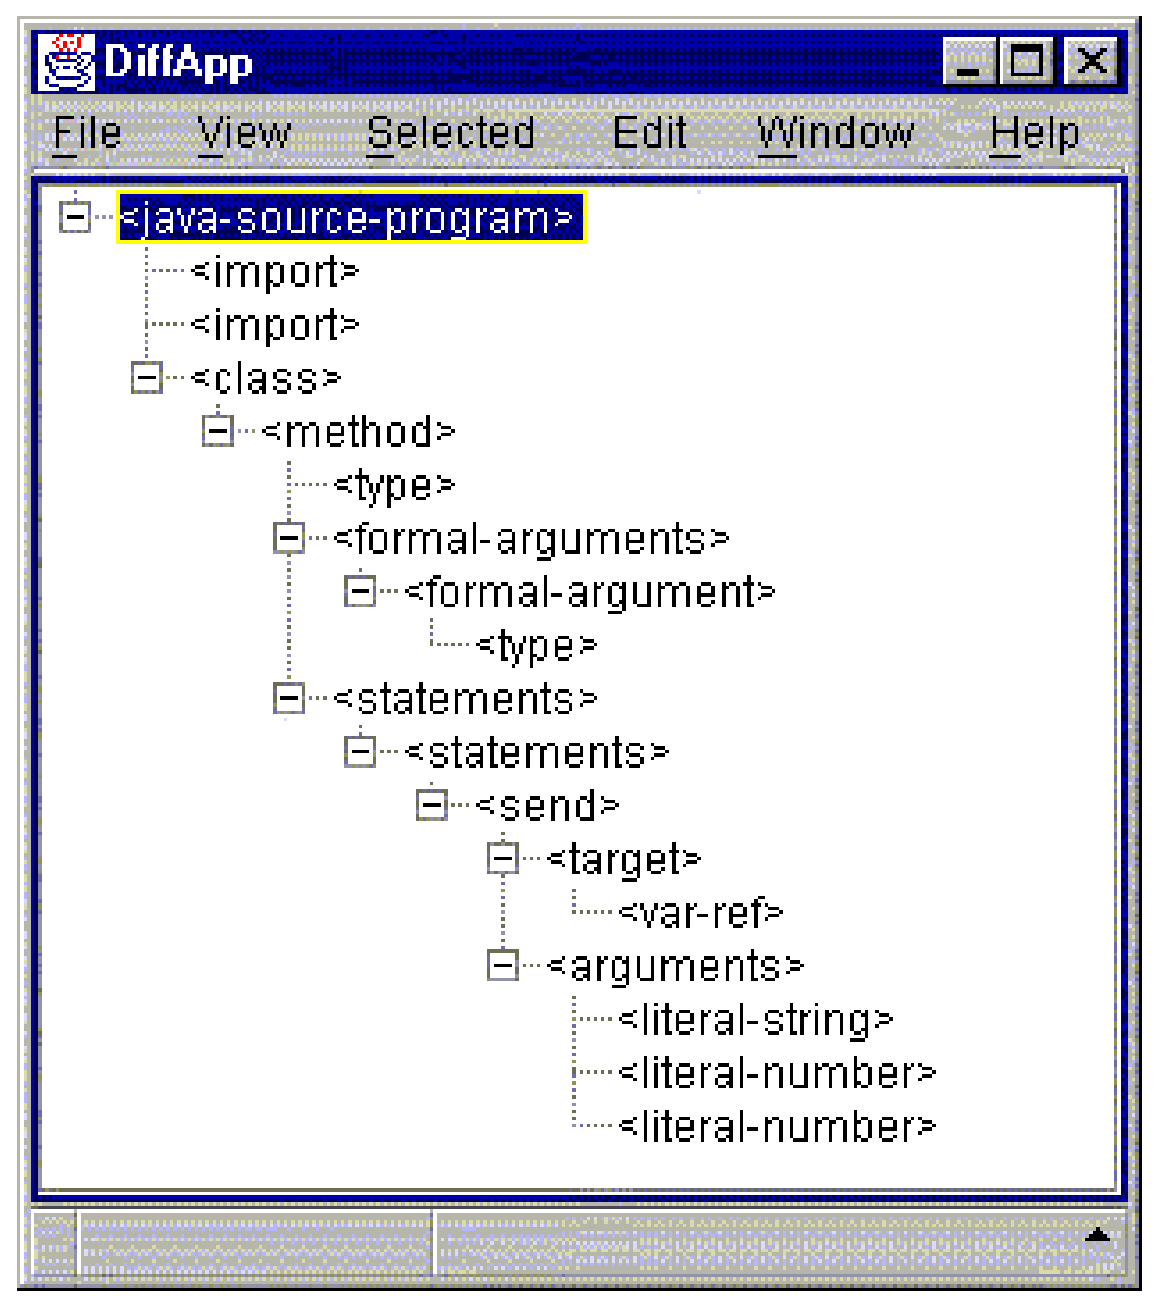
\includegraphics[width=\linewidth]{treeview.eps}
\caption{A fully-expanded tree view of the JavaML representation 
of the \smtexttt{FirstApplet} example as viewed by IBM's
\smtexttt{xmldiff} utility~\cite{XMLDiffMerge}.
\label{fig-treeview}}
\end{centering}
\end{figure}

\subsection{Design decisions}
\label{ssec-design}

JavaML provides more than just the structure of the source program,
though.  In the preceding example, notice the use of the formal-argument
\smtexttt{g} in line 17 as the target of the message send.  The
\smtexttt{idref} attribute of that \smtexttt{var-ref} tag points back at
the referenced \smtexttt{formal-argument} element (through its
\smtexttt{id} attribute).  (The \smtexttt{id} value chosen for a
to-be-referenced element must be unique within a document so each
identifier is branded with an integer to keep the values distinct.)
This linking is standard XML, thus XML tools are able to trace from a
variable use to its definition to, e.g., obtain the type of the
variable.  Similar linking is done for local (block-declared) variables.
In JavaML, variable references are easy to locate because of their
distinguishing \smtexttt{var-ref} tag.  Additionally, they are
disambiguated from an assignment to a variable which is converted into a
\smtexttt{var-set} tag.

Throughout JavaML, attributes of elements are used whenever the
structure of the value can never be more complex than a simple text
string.  Attributes are used for modifiers such as
\smtexttt{synchronized} and \smtexttt{final} and for visibility settings
such as \smtexttt{public} or \smtexttt{private}.  Attributes are not
used for properties such as types because types have some structure: a
type can consist of a base name and a number of dimensions, and could
also reference the definition of the class that implements the type, if
desired.  If, say, a return type were just the value of an attribute on
the method element, the end user would unacceptably have to do string
processing on the attribute's value "\smtexttt{int[][]}" to determine
that the base type of that two-dimensional array was the primitive type
\smtexttt{int}.  Instead, types are modeled as explicit child elements
such as \smtexttt{<type name="int" dimensions="2">}.

JavaML generalizes related concepts to simplify some analyses but also
preserves distinctions that may be needed for other tasks.  For example,
\smtexttt{45} and \smtexttt{1.9} are represented as:
\smtexttt{<literal-number kind="integer" value="45">} and
\smtexttt{<literal-number kind="float" value="1.9">}, respectively.  An
alternate possible markup is: \smtexttt{<literal-integer value="45">}
and \smtexttt{<literal-float value="1.9">} but using separate element
classes eliminates the tight relationship that both values are numbers
and can complicate using the representation.  Instead, we use a single
element tag and disambiguate these literals based on a \smtexttt{kind}
attribute. Thus, we can still tell the difference between a floating
point literal and an integer literal, but in the common case we gain the
same flexibility of numeric types that the Java language has.

Another place where JavaML generalizes language constructs is loops.
Both \smtexttt{for} and \smtexttt{while} loops can be viewed as general
looping constructs with 0 or more initializers, a guarding test that
occurs before each iteration, 0 or more update operations, and a body of
statements that comprise the looped-over instructions.  Thus, instead of
using two classes of elements, \smtexttt{for-loop} and
\smtexttt{while-loop}, JavaML uses a single \smtexttt{loop} element that
has a \smtexttt{kind} attribute with value either \smtexttt{for} or
\smtexttt{while}.  When a \smtexttt{while} loop is converted, it will
have neither \smtexttt{initializer} nor \smtexttt{update} children, yet
a \smtexttt{for} loop could potentially contain many of each.  In
contrast, distinct \smtexttt{do-loop} elements are used for
\smtexttt{do} loops because they have their test performed at the end of
the loop, instead of at the start.

%% Talk about unparsing loops kind="while" w/ initializer? [as result
%% of transformation, say] We definitely can do it, and it's pretty cool
      
As yet another example, we represent both instance and class (i.e.,
static) fields as \smtexttt{field} elements with a \smtexttt{static}
attribute used to disambiguate.  Although there are more substantial
differences between these two concepts than between \smtexttt{while}
and \smtexttt{for} loops, it still seems beneficial to use a single
kind of element for both kinds of fields.

Local variable declarations provide a syntactic shorthand that raises an
interesting question about their underlying representation.  The code
segment \smtexttt{int dx, dy;} defines two variables both of type
\smtexttt{int}, but with perhaps a subtle additional intention: that the
two variables have the same type.  For contrast, consider \smtexttt{int
  weight, i;}.  Here, there probably is \emph{not} the implicit desire
that the two variables have the same type, but instead the shorthand
syntax is being used simply for brevity.  Because it is hard to automate
distinguishing these cases, JavaML simply preserves this syntactic
feature by using a \smtexttt{continued="true"} attribute on variable
declarations that exploit this shorthand.

The careful reader will observe that the JavaML representation is about
three times longer than the classical source code.  That expansion is a
fundamental tradeoff of moving to a self-describing data format such as
XML.  It is important that the terse classical representation can be
employed by programmers in certain tasks including ordinary development
and program editing.  JavaML is complementary to the classical source
representation and is especially appropriate for tools, though it is
still accessible and readable to developers.

\subsection{Implementation of converter}

To experiment with the design of JavaML and gain experience in using the
representation, it was essential to implement a converter from the Java
classical source representation to JavaML.  Within the IBM Jikes Java
compiler framework~\cite{Jikes}, I added an \smtexttt{XMLUnparse} method
to each of the AST nodes. This change, along with some small additional
code for managing the options to request the XML output, results in a
robust and fast JavaML converter.  In total, I added about 1600
non-comment-non-blank lines of C++ code to the Jikes framework to
support the option.  The source code is available upon request (and will
be made publicly available shortly after final submission of this
paper).

The converter has been tested by converting several sample programs, as
well as the whole of the 4300 line Cassowary Constraint Solving
Toolkit~\cite{CassoInI}.  The processing of all those files takes only
about six seconds on the author's RedHat6-based dual Pentium III-450
machine.  Each of the files converted was then validated with respect to
the JavaML DTD using James Clark's Jade package's \smtexttt{nsgmls}
tool~\cite{Jade}.

Also implemented is a prototype back-converter that outputs the
classical source representation given the JavaML representation. That
application uses the XML and DOM packages and contains about 360 lines
of Perl.  See section~\ref{sec-future} for more details about
back-converting possibilities.

\section{Leveraging XML}
\label{sec-leveraging}

JavaML uses XML as an alternate, structured representation of a Java
source program.  Although the abstraction away from syntactic details of
Java is convenient, the more important benefit is that JavaML enables
the use of the rich infrastructure developed to support SGML and XML.
Instead of building analysis and transformation tools from scratch to
work on a proprietary binary structured format for a program, existing
SGML and XML tools can be used, combined, and extended.  XML tools
encompass a broad range of features that include querying and
transformation, document differencing and merging~\cite{XMLDiffMerge},
and simple APIs for working with the document directly.  In this paper,
I will (for space reasons) limit discussion to uses of only three tool
groups:

\begin{itemize}
\item the XML toolbox (ltxml) from Edinburgh University~\cite{ltxml}
which contains \smtexttt{sgcount},
\smtexttt{sgrpg}, \smtexttt{sggrep}, and more;

\item the perlSGML utilities~\cite{perlSGML} which
contains \smtexttt{dtd2html}, \smtexttt{dtddiff},
\smtexttt{dtdtree}, and more; and

\item the Perl XML::DOM package~\cite{perlDOM} which exposes a
DOM level~1~\cite{DOM} interface to an XML tree.
\end{itemize}

These are just a very small subset of the tools that prove useful when
working with JavaML.  In the following examples, we will query the
\smtexttt{Set.java.xml} document that appears in
appendix~\ref{app-ext-eg}.  Although these examples are small by
real-world standards, XML and SGML tools target documents ranging up
through lengthy books so the implementations are designed to scale well.

One common software engineering task (for better or for worse) is to
accumulate metrics about a source code artifact.  With JavaML, the SGML
utility \smtexttt{sgcount} does an excellent job of summarizing the
constructs in a Java program:

%% ShellCommand
{\bfseries
\begin{verbatim}
% sgcount Set.java.xml
\end{verbatim}
}
{\small
\begin{verbatim}
new                    5  
method                 9  
lvalue                 4  
if                     1  
var-set                4  
literal-true           2  
assignment-expr        4  
loop                   1  
formal-argument        7  
package-decl           1  
local-variable         2  
literal-null           2  
target                 18 
cast-expr              1  
constructor            4  
arguments              23 
import                 1  
send                   18 
return                 8  
test                   2  
formal-arguments       13 
class                  1  
java-source-program    1  
true-case              1  
type                   25 
conditional-expr       2  
var-ref                25 
literal-false          2  
statements             25 
literal-string         3  
binary-expr            3  
field                  1  
*Total*                219 
\end{verbatim}
}

In the above output, each row lists an element class and the number of
times that that element appeared in the document.  Thus, we can easily
see that there are 9 \smtexttt{method} elements, thus there are 9
method definitions.  Similarly, we can see that there is 1 class
definition, 25 variable references, 18 message sends, and 3 string
literals.  This summary is far more indicative of the content of a
program than a typical lexical measure such as the number of lines of
code.

Suppose we wish to see all the string literals that a program contains.
We can do this trivially using \smtexttt{sggrep} on the JavaML
representation of the program:

\begin{verbatim}
% sggrep '.*/literal-string' \
           < Set.java.xml
\end{verbatim}

{\small
\begin{verbatim}
<?xml version='1.0' encoding='UTF-8'?>
<!DOCTYPE java-source-program SYSTEM "java-ml.dtd" >
<literal-string length='2'>{ </literal-string>
<literal-string length='2'>, </literal-string>
<literal-string length='4'> }\n</literal-string>
\end{verbatim}
}

\noindent Notice that the output of \smtexttt{sggrep} is also a (not necessarily
valid nor even well-formed) XML document.  Thus we can string together
SGML and XML tools in a Unix pipeline to combine tools in novel and
useful ways.  For example, if we want to just see the strings, we can
run \smtexttt{stripsgml} on the output of the above query:

\begin{verbatim}
% sggrep '.*/literal-string' \
           < Set.java.xml | stripsgml
\end{verbatim}

\begin{verbatim}
{ 
, 
 }\n
\end{verbatim}

We can also query the JavaML source for elements based on values of
their attributes.  For example, if we wish to find all sends of the
message \smtexttt{clone} we can do so easily and reliably:

\begin{verbatim}
% sggrep '.*/send[message=clone]' \
                      < Set.java.xml 
\end{verbatim}

{\small
\begin{verbatim}
<?xml version='1.0' encoding='UTF-8'?>
<!DOCTYPE java-source-program SYSTEM "java-ml.dtd" >
<send message='clone'>
<target>
<var-ref name='hash'/>
</target>
<arguments/>
</send>
\end{verbatim}
}

Another class of common analyses is the semantic checks done by the
compiler prior to translation.  For example, in Java code, only abstract
classes may have abstract methods.  When compiling, a semantic error
will be flagged if this rule is violated.  We can query a JavaML document
for concrete (i.e., not abstract) classes that contain an abstract method:

{\small
\begin{verbatim}
% sggrep -q '.*/class[abstract!=true]/\
                method[abstract=true]' \
                          < Set.java.xml
\end{verbatim}
}

\noindent and the output will be empty because this semantic restriction is not
violated in our target document (i.e., the analyzed program).

A common error for novice Java programmers is to accidentally use the
assignment operator, \smtexttt{=}, instead of using the equality test
operator, \smtexttt{==}.  Although the Java type checker will catch
most of these errors at compile time, it will miss the problem if
the assigned-to variable is a \smtexttt{boolean}. If we wish to find these
questionable constructs, \smtexttt{sggrep} makes this analysis
trivial thanks to the JavaML representation:

{\small
\begin{verbatim}
% sggrep -q '.*/if/test/assignment-expr' \
                            < Set.java.xml
\end{verbatim}
}

\noindent The \smtexttt{sgrpg} (SGML RePort Generator) program permits combining a
top-level query with a restriction on the children and an output format
for the results (a common paradigm for querying tools~\cite{XMLQL-EnE}.
For example:

{\small
\begin{verbatim}
% sgrpg '.*/method' \
        '.*/send[message=hasMoreElements]' \
        '' '%s %s 
' visibility name < Set.java.xml
\end{verbatim}

\begin{verbatim}
public toString
\end{verbatim}
}

\noindent searches for method definitions that contain message sends of the
message \smtexttt{hasMoreElements}.  It then outputs the
\smtexttt{visibility} and \smtexttt{name} attributes of the matched
elements as shown above.

A wide variety of analyses are possible just using the querying
capabilities provided by standard XML tools.  Other things we can find
are returns from inside for loops, all definitions of integer variables,
string variables that do not conform to our project's naming convention,
and much more.

Transformations on source code are also very useful when modifying and
evolving software artifacts.  Obviously, querying tools can only prune
elements from the source document or combine elements from multiple
documents.  More powerful transformations are possible using
XSLT~\cite{XSLT}, DSSSL~\cite{DSSSL}, or directly manipulating the
document using a DOM (Document Object Model)~\cite{DOM} interface.  For
example, we can rename methods named \smtexttt{isBall} to
\smtexttt{FIsBall} using the Perl package \smtexttt{XML::DOM} and the
following in the \smtexttt{start\_tag} subroutine:

\begin{verbatim}
sub start_tag { 
  my ($this,$tag,$attr_spec) = @_;
  my $from = "isBall";
  my $to = "FIsBall";
  my %attrs = 
     SGMLparse_attr_spec($attr_spec);
  # ...
  if ($tag eq "method") {
    if ($attrs{name} eq $from) {
      $attrs{name} = $to;
    }
  } elsif ($tag eq "send") {
    if ($attrs{message} eq $from) {
      $attrs{message} = $to;
    }
  }
  # ...
}
\end{verbatim}

Other possibilities for transformations include using a style sheet to
convert from JavaML back into the classical source representation or a
PostScript text representation with nice syntax highlighting.  Adding
debug or instrumentation code at entry and exit to and from functions is
also straightforward.

\section{Related work}
\label{sec-related}

A key benefit of JavaML is its ability to leverage the growing
infrastructure of SGML and XML related tools and techniques as described
in the previous section.  Various researchers have similarly approached
the problem of improving software engineering and development tools with
varying degrees of success.

TAWK~\cite{Griswold96} extends the AWK~\cite{Dougherty90} paradigm by matching
patterns in the AST of a C program.  Numerous XML querying tools provide
this same functionality for JavaML, and the event-action framework is
similar to that used by SAX (Simple API for XML)~\cite{SAX}.

ASTLog~\cite{Crew97} extends the Prolog~\cite{Clock94} logic programming
language with the ability to reason about an external database that
models the AST.  Unlike Prolog, ASTLog statements are evaluated with
respect to a current object.  The approach that Crew uses may be
interesting to apply to the XML world, but the numerous XML tools
already provide comparable functionality through a more conventional (if
perhaps less convenient) framework.

CCEL~\cite{CCEL92} provides a metalanguage for expressing non-linguistic
intentions (i.e., ones that cannot be expressed in the language) about
software artifacts written in C++.  JavaML can provide a similar
capability by simply writing queries that search for violations of the
intended invariants and reporting them as part of the edit, build, or
regression-test procedure throughout the development cycle.

Microsoft's Intentional Programming group~\cite{Simonyi96} has long been
working on a more abstract representation of computation that is
syntax-independent.  Their goal appears to be to permit developers to
describe new abstractions along with techniques to reduce those
abstractions down to known primitives.  In essence, they are interested
in permitting the developer to grow a domain-specific language as they
build their software.  JavaML is especially exciting as a representation
for this approach.  We can view new abstractions as incremental
extensions to DTDs.  In order for the new document type, call it
Java++ML, to still be compilable by a stock Java compiler, the developer
must simply write a transformation from Java++ML to JavaML.  Because
DTDs are exceptionally easy to extend, this approach is tenable and
likely a fruitful avenue for future work.  There are several utilities
for documenting and comparing DTDs (e.g., \smtexttt{dtd2html} and
\smtexttt{dtddiff}) that would be helpful when applying this technique.


\section{Future work}
\label{sec-future}

The one unfortunate shortcoming of the current implementation of the
classical source representation to JavaML converter is that it loses
source-level comments.  Although these are an essential part of any
software artifact, conventional parsing technology throws the comments
away early in the lexical analysis phase.  Because the comments are
never a part of the internal representation of the program inside the
Jikes compiler framework, they cannot be unparsed into JavaML.  Even
after modifying the compiler's internal representation to support
comments, there will remain the problem of choosing to what element to
attach a given comment.  Although this is a hard problem, the JavaDoc
conventions for documenting source code will simplify properly attaching
a large fraction of the comments.

Another useful extension to the current transformation system is to do
more cross-linking of elements.  Type elements could reference their
defining classes in other JavaML documents.  Import declarations could
reference the top-level documentation for the imported package.  Many
more possibilities are imaginable.

JavaML should be refined to guarantee that it is a complete, isomorphic
representation of the constructs present in the latest version of the
Java programming language.  Additionally, it is likely beneficial to
migrate JavaML to use XML Schema~\cite{XMLSchema1,XMLSchema2} instead of
a DTD after the Schema working drafts are finalized.

Although this paper has presented a markup language for Java, the same
basic approach can be applied to other programming languages, or even to
translate among languages.  To the extent that the representation
abstracts away syntax, JavaML may also prove useful in permitting the
import of visual representations such as Unified Modeling Language
diagrams~\cite{UMLNutshell,XMI}.  Certainly generating visual
representations of important properties of software artifacts is on the
immediate horizon given the capabilities of XSL and DSSSL.

One significant complication in applying this approach to C++, another
popular conventional object-oriented-programming language, is the C
preprocessor.  The C preprocessor provides a first pass of textual
processing to permit abstractions that cannot otherwise be expressed in
the core C++ language.  These abstractions are often very important to
the understandability and maintainability of the code, but do not
interact well with parsing techniques~\cite{ErnstBadrosNotkin00,Badros00-spe}.

The current converter that translates back from JavaML to the classical
source representation needs to be far more robust.  It was written as
only a proof of concept and for the author to gain experience with the
XML DOM.  A better approach is to add a Jikes front-end that uses an XML
parser (e.g., XML4C++~\cite{XML4C++}) to construct the XML DOM from the
JavaML source, then simply write a recursive conversion function to
build the Jikes internal AST from using the DOM API.  Then, using
Jikes's pre-existing conventional unparser, the compiler can write out
the classical representation for the source code.  The key benefit of
this technique is that it then permits the compiler to work directly on
the JavaML representation of the source code via the new front-end.

Using JavaML as the primary source representation has the potential to
simplify the compiler beyond just eliminating its classical front-end.
Some semantic analyses can be removed from the compiler once it knows
that the input is a valid JavaML document.  It will be useful to
characterize which semantic errors are provably impossible to encounter
given that precondition.  Additionally, more semantic analyses can be
moved into the editing environment reasonably painlessly in the form of
straightforward queries (such as some of those described earlier in
section~\ref{sec-leveraging}).

Because the concise textual representation of source code is nicely
suited to expert programmers, it's unlikely that they will be interested
in discarding their favourite text editor anytime soon.  It will be
useful to investigate better ways to convert interactively and
incrementally from the classical source representation to JavaML and
support useful editing capabilities along the lines of current text
editing systems.  The work on structured text editors is highly relevant
here, but may prove more fruitful given the incredible resources that
can now be thrown at the problem given the growing commercial importance
of XML technology.

\section{Conclusion}
\label{sec-conclusion}

JavaML is an alternate representation of Java source programs that is
based on XML.  Unlike the classical textual source representation, the
JavaML representation makes it easy for software tools to reason about
programming-level constructs in a Java program.  This benefit results from the
ability of JavaML to more directly represent the structure of the program.

Given JavaML, the wealth of pre-existing XML and SGML tools can perform
numerous interesting and useful analyses and transformations of Java
source programs.  XML tools are improving continually to support the
growing infrastructure of XML-based documents.  Ultimately, JavaML could
replace the classical source representation of Java programs as the
storage format for programs, relegating text-parsing to just one of many
possible ways of interacting directly with the structured representation
of the software artifact throughout the development process.

\section*{Acknowledgments}
\label{sec-ack}

I enthusiastically thank Zack Ives for his comments, discussion, and
input on this work.  I thank Corin Anderson and Alan Borning for
much-appreciated comments on a draft of this paper.  I also thank Miguel
Figueroa, Craig Kaplan, and Todd Millstein, and Stefan Bjarni Sigurdsson
for their helpful discussions. Thanks to IBM for constructing the Jikes
compiler framework, and for making it publicly available, and thanks to
Mike Ernst for helpful pointers on using it. This work was supported by
the University of Washington Computer Science and Engineering Wilma
Bradley fellowship and by NSF Grant No. IIS-9975990.

\appendix
\section{JavaML DTD}
\label{app-javaml-dtd}

{\small
\verbatiminput{java-ml.dtd-formatted}
}

\end{multicols}

\section{Extended Example}
\label{app-ext-eg}

\subsection{Set.java}

{\small 
\verbatiminput{Set.java} 
}


\subsection{Set.java.xml}
{\small
\verbatiminput{Set.java.xml} 
}

\begin{multicols}{2}

{\small
\bibliography{library,articles,applications} %style plain, from above.
}

%% GJB:FIXME:VISUAL
%\vspace{2in}

\section*{Vitae}
\begin{floatingfigure}[l]{.9in}
\hspace*{-.6cm}

\includegraphics[width=1in]{gjb-face.eps}
\end{floatingfigure}
%%<a href="http://www.cs.washington.edu/homes/gjb">
\textbf{Greg J. Badros} is a final-year Ph.D. candidate at the
%% <a href="http://www.cs.washington.edu">
University of Washington in Seattle, USA where he earned his
M.Sc.\  degree in 1998.  He graduated \textit{magna cum laude} with a B.S.
degree in Mathematics and Computer Science from
%% <a href="http://www.math.duke.edu">
%% <a href="http://www.cs.duke.edu">
%% <a href="http://www.duke.edu">
Duke University in 1995.  He is the primary author of the 
%% <a href="http://scwm.mit.edu">
Scheme Constraints Window Manager and the 
%% <a href="http://www.cs.washington.edu/research/constraints/cassowary/">
Cassowary Constraint Solving Toolkit.  His research interests include
constraint technology, software engineering, languages, and the
Internet.
\end{multicols}


\end{document}

%%% Local Variables: 
%%% mode: latex
%%% TeX-master: t
%%% End: 
